\chapter{Конструкторский раздел}
\label{cha:design}

В данном разделе будет представлена схема алгоритма шифрования AES.

\section{Алгоритм шифрования AES}

На рисунке \ref{fig:des01} изображена структурная схема шифрования AES.


\begin{figure}[H]
	\centering
	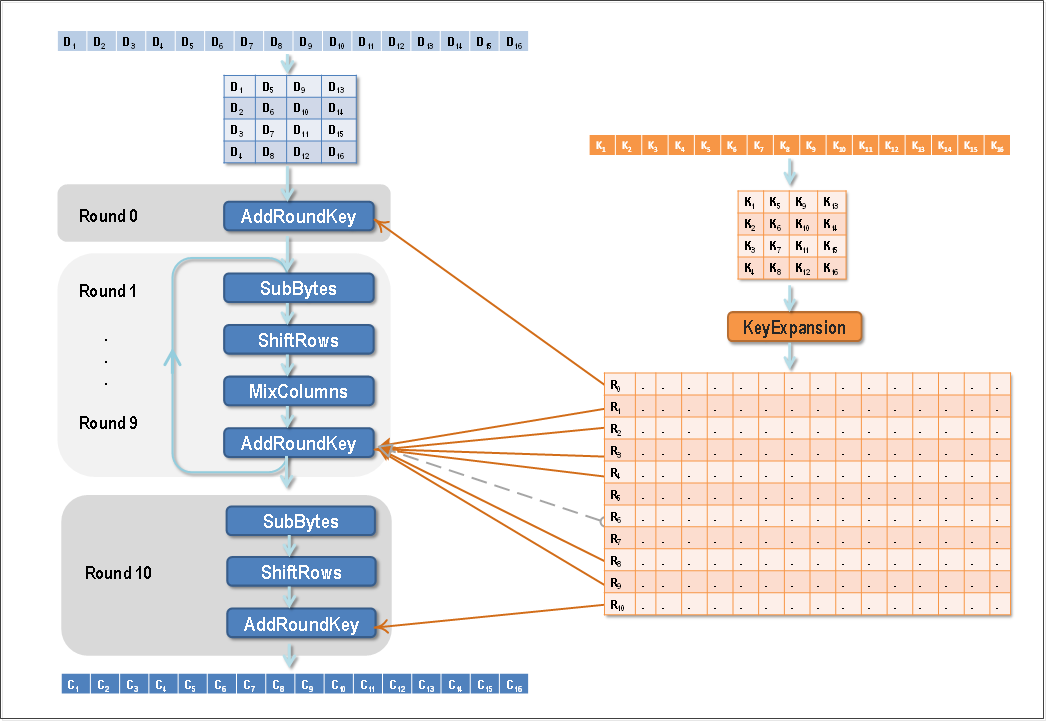
\includegraphics[width=1\linewidth]{img/aes_gen}
	\caption{Структурная схема шифрования AES}
	\label{fig:des01}
\end{figure}

На рисунке \ref{fig:des3} изображена схема блока SubBytes.

\begin{figure}[H]
	\centering
	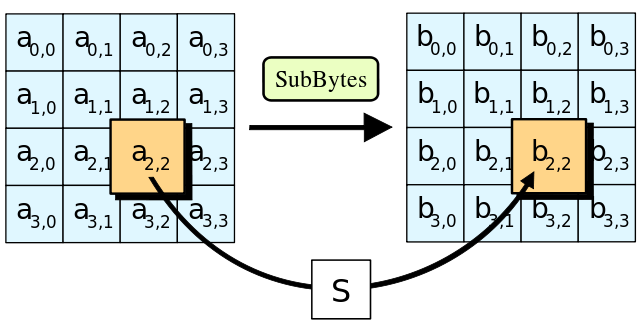
\includegraphics[width=0.7\linewidth]{img/aes_subb}
	\caption{Схема блока SubBytes}
	\label{fig:des3}
\end{figure}

На рисунке \ref{fig:des4} изображена схема блока ShiftRows.

\begin{figure}[H]
	\centering
	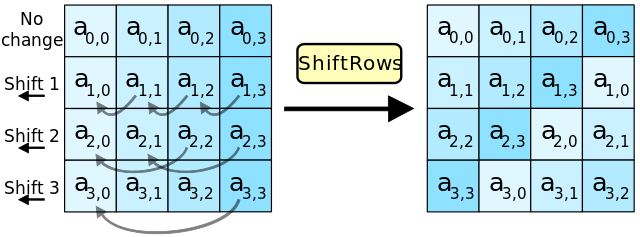
\includegraphics[width=0.7\linewidth]{img/aes_shiftr}
	\caption{Схема блока ShiftRows}
	\label{fig:des4}
\end{figure}

На рисунке \ref{fig:des5} изображена схема блока MixColumns.

\begin{figure}[H]
	\centering
	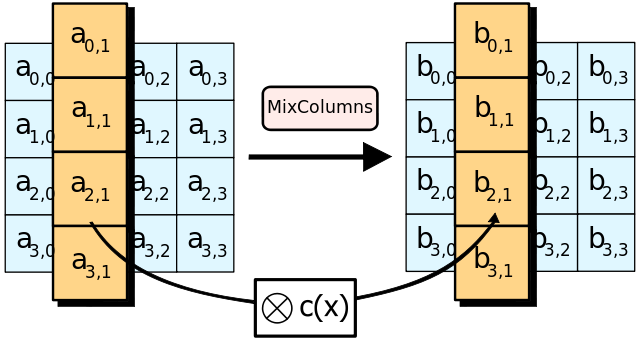
\includegraphics[width=0.7\linewidth]{img/aes_mixc}
	\caption{Схема блока MixColumns}
	\label{fig:des5}
\end{figure}

На рисунке \ref{fig:des6} изображена схема блока AddRoundKey.

\begin{figure}[H]
	\centering
	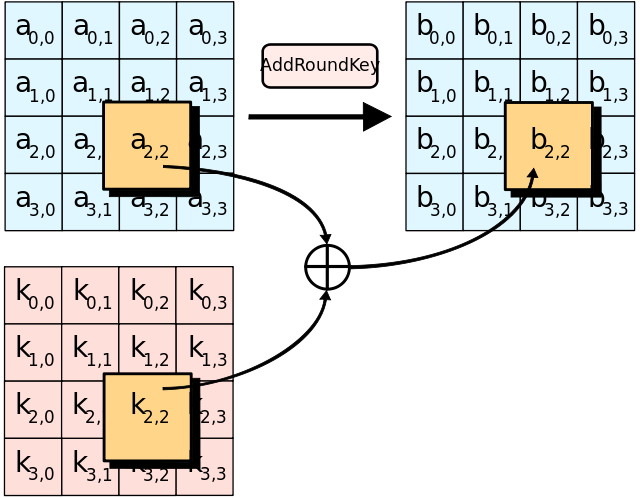
\includegraphics[width=0.7\linewidth]{img/aes_roundk}
	\caption{Схема блока AddRoundKey}
	\label{fig:des6}
\end{figure}

На рисунке \ref{fig:des7} изображена структурная схема блока KeyExpansion.

\begin{figure}[H]
	\centering
	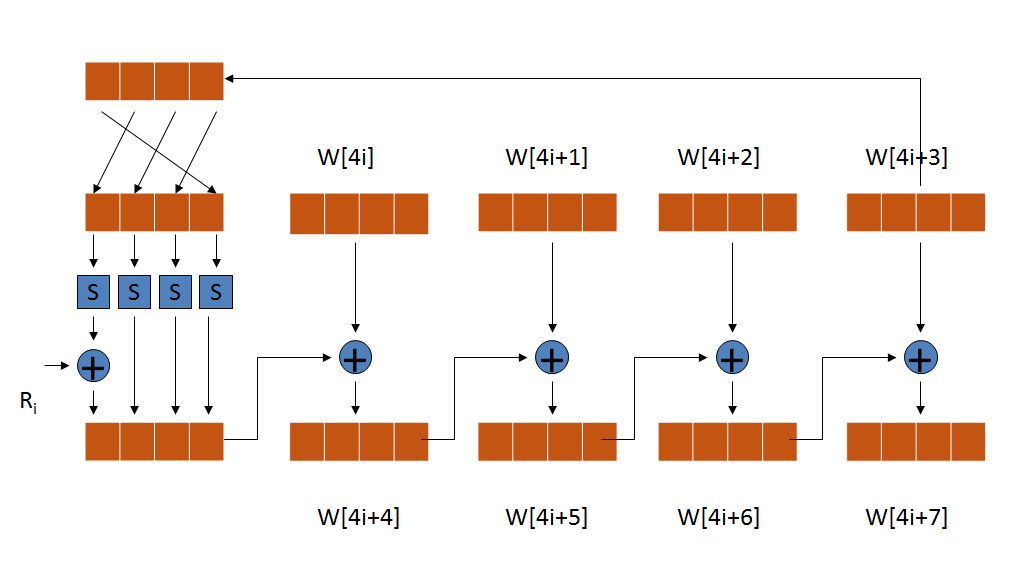
\includegraphics[width=0.7\linewidth]{img/aes_keys}
	\caption{Структурная схема блока KeyExpansion}
	\label{fig:des7}
\end{figure}

\section*{Вывод}
В данном разделе были приведены структурные схемы шифрования AES.


